
\chapter{用户兴趣探索}
\section{引言}
\label{chap:interestExplore}
电子商务产品的设计往往是数据驱动的,即许多产品方面的决策都是把用户行为数据量化后得出的。但就小米主题市场而言,只有那些热门主题才有足够多的数据可以挖掘,大部分主题只有很少的数据可供分析、挖掘,因此,需要一种方法对用户行为做针对性挖掘,利用少量数据获得出用户真正的偏好度,最终提升商品的销售量,这是问题之一。现有的推荐算法注重用户静态属性的同时却忽略了用户兴趣的动态变化,从而导致系统在时间维度上有偏离用户需求的趋势,这是问题之二。用户兴趣探索模块可以很好的解决此类问题。

探索用户兴趣的数据来源包括用户行为数据、用户画像和商品特征表。用户画像包括用户基本信息和兴趣标签等,商品特征表包括分类、属性标签等,过程分为几个步骤:首先,利用用户历史行为(评论,停留时长,评分,点赞,购买等)量化用户满意度,然后利用用户兴趣特征向量与商品特征矩阵得出相关分数,如果商品与用户的相关分数很低,但有很高的用户满意度,说明是一次成功的用户兴趣探索,更新用户画像。如果是热门商品,大量的用户都会点击,但商品与用户不是很相关,则认为其探索效果是有限的,反之如果是小众商品,考虑到长尾效应,则可以认为其是更成功的兴趣探索。这里涉及到的概念包括用户满意度的量化、用户和商品的关联度、商品属性标签的长尾性,下文会一一给出详细说明。

\section{用户行为数据的存储和处理}
手机主题用户行为数据的特点包括:1、用户基数庞大,手机主题注册用户达千万级,活跃用户达百万级。2、用户规模增长快,月新注册用户达10万数量级。3、每个用户的行为数量较小,即使是活跃用户,每天最多也只产生上百条行为记录。4、用户行为的计算较为复杂,计算用户的两次登录间隔天数、反复购买的商品、累积在线时间,这些都是针对用户行为的计算,通常具有一定的复杂性。5、用户行为数据格式不规整,字段丢失率较高。

  \subsection{数据预处理}
  数据预处理是数据挖掘过程中一个重要步骤,主要工作包括字段去重、无效日志过滤、多表字段的连接等。如统计2015年09月06号userId为001的投诉数,数据预处理过程如\autoref{code:data-predoing}。
  \begin{lstlisting}[language=java,firstnumber=1,label={code:data-predoing}, caption={数据预处理脚本}]
    set hiveconf:ymdwithline=2015-09-06;
    set hiveconf:metric=complaint_order_num;
    set hiveconf:user_id=001;

    select '${hiveconf:metric}' as metric, count(a.order_id) as score
    from (
        //去重
        select distinct order_id
        from theme.dw_v_order_base
        //以时间范围date_sub('${hiveconf:ymdwithline}',5) and '${hiveconf:ymdwithline}'为条件过滤掉不符合条件的订单
        where concat_ws('-',year,month,day) between date_sub('${hiveconf:ymdwithline}',5) and '${hiveconf:ymdwithline}'
        //无效订单过滤
        and order_id!=null
        //以用户id为条件过滤掉其他订单
        and user_id=${hiveconf:user_id}
    ) a
    inner join (
        //order_id 字段去重
        select distinct order_id
        from theme.g_comment_complaint
        //type = 3表示用户投诉
        where concat_ws('-',year,month,day) = '${hiveconf:ymdwithline}' and type = 3
        //多表字段的连接,如果有一个表有投诉记录,就算一次投诉。
        union
        select distinct order_id
        from theme.dwd_kefu_phone_complaint
        where concat_ws('-',year,month,day) = '${hiveconf:ymdwithline}'
    ) b
    on a.order_id = b.order_id
    group by metric;
  \end{lstlisting}

\section{用户兴趣探索模型}
用户兴趣探索主要功能模块包括:1,兴趣标签探测,在分析用户行为数据时,如果某些主题标签和用户相关度很低,那么这些标签会作为标签探索候选集。2,长尾标签提取,基于小众标签集,按照某种规则筛选出目标标签。3,用户满意度量化,根据用户所有对某一个主题的行为数据得出这个用户对这个主题的满意度。4,标签权重的更新,不管是不是一次成功的兴趣标签探索,都要对用户画像标签的权重做更新,更新算法利用了线性衰减思想。本章首先介绍一些基本概念,包括实体域、用户行为和用户满意度等。然后详细介绍用户兴趣探索功能模块的实现。
  \subsection{基本概念概述}
  实体域。如果一个模型是基于分析用户行为得出用户兴趣时,实体就是这个行为针对的对象。不同实体通过标签关联起来,对于手机主题应用市场来说,实体域还包括所有的背景图片,铃声,闹铃等。

  用户行为。包括浏览,点击,下载,试用,购买,评论。本文所指的用户行为都是指用户在某手机主题上的行为。

  用户满意度。用户满意度是指根据用户作用在主题上的不同行为动作及其属性值,反推得到的用户偏好度。

  小众标签集。小众标签集是指用户偏好频率低的主题标签的集合,需要补充是,长尾标签和小众标签大多数是一致的,只是长尾标签针对商品而言,小众标签针对用户而言。

  \subsection{兴趣标签探测功能模块}
  首先候选标签是与用户相关度低的标签,如用户001每次都会浏览动漫、美少女主题,但是有一天却购买了一款汽车手机主题,通过计算发现汽车标签对于用户001是从未遇到过的标签,即相关度为0,于是汽车标签将会是潜在的探索标签。事实上用户兴趣探索过程可以在很短的时间内完成,基于 Hive + HDFS 平台的时长维度为天,而基于 Kafka + Spark 平台可以将时长维度降到小时级别。

  \subsection{长尾标签抽取功能模块}
  首先需要介绍标签集中度(tagFocus)和标签热度(tagPopular),标签集中度针对商品而言,标签热度针对用户而言。

  标签集中度。如果某一类主题包集合中包含某兴趣标签的个数为tagInThemeNum,而其它类包含的总数为tagInOtherNum,当tagInThemeNum大的时候,就说明其集中度高。实际上,如果一个标签在同一类主题集合中频繁出现,则说明该标签能够很好代表这类主题集合的特征,这样的标签应该给它们赋予较高的权重,并选来作为该类主题的特征向量以区别于其它类主题,标签集中度公式如\autoref{equ:focus},我们很容易发现,如果一个标签只出现若干主题包,我们通过它就容易定位搜索目标,因此其权重也应该大。反之如果一个词在大量主题包中出现,其权重取较小为好。
  \begin{equation}
    tagFocus=\frac{|tagInThemeNum|}{|tagInThemeNum+tagInOtherNum|}
    \label{equ:focus}
  \end{equation}

  标签热度。标签热度指的是某一个给定标签在用户画像中出现的频率。例如在300万用户总数中,十分之一的用户标签中有“火影”标签,那么其热度为0.1。标签热度不是越大越好,有些标签如“精品”,“气质”等标签占了总词频的80\%以上,而它对区分主题类型几乎没有用,我们称这种词叫“应删标签”。即应删除词的权重应该是零,也就是说在度量相关性是不应考虑它们的频率。

  长尾标签定义为集中度和热度之比大于一个给定阈值的标签,且本身为小众标签。代码如\autoref{code:longtail-tag}。
  \begin{lstlisting}[language=java,firstnumber=1,label={code:longtail-tag}, caption={长尾标签抽取算法}]
    public Set<String> getLongTailTags(String userId, String itemId) throws Exception {
        Set<String> out = new HashSet<>();
        //获取所有小众标签
        HashSet<String> longTailTags = getColdTags();
        //获取所有当前用户画像没有的标签
        Set<String> rawTags = tagExplore(userId, itemId);
        for (String tag : rawTags) {
            if (!longTailTags.contains(tag)) {
                continue;
            }

            //获取标签的集中度
            long tagFocusScore = getTagFocusScore(tag);
            //获取标签的热度
            long tagPopularScore = getTagPopularScore(tag);
            if (tagFocusScore / tagPopularScore <= threshold) {
                continue;
            } else {
                out.add(tag);
            }
        }

        return out;
    }
  \end{lstlisting}

  \subsection{用户满意度量化功能模块}
    \autoref{tab:userAction}列举的用户行为包含了部分关键的行为类型,通过将不同行为反映为用户喜好的不同并进行加权累积,得到用户对于物品的总体喜好。显式的用户反馈比隐式的权值大,但比较稀疏,毕竟进行显示反馈的用户是少数;而隐式用户行为数据是用户在使用应用过程中产生的,它可能存在大量的噪音和用户的误操作,通过数据挖掘算法滤掉可能的噪音,这样使分析更加精确。然后是归一化操作,因为不同行为的数据取值可能相差很大,比如,用户的浏览数据必然比购买数据大的多,如何将各个行为的数据统一在一个相同的取值范围中,从而使得加权求和得到的总体喜好更加精确,就需要进行归一化处理使得数据取值在 [0,10] 范围中。

    \begin{table}[htp]
    \centering
    \tabcaption{用户行为权重对应表}
    \label{tab:userAction}
    \begin{tabular}{ |c|c|p{4cm}|p{5cm}|c|} \hline
     用户行为 & 类型 & 特征 & 作用 & 权重\\ \hline
     评分 & 显式 & 整数量化的偏好,可能的取值是 [0,5] & 通过用户对物品的评分,可以精确的得到用户的满意度,但是噪声比较大,比如遇到好评返现活动 & 1\\ \hline
     分享 & 显式 & 布尔量化的偏好,取值是 0 或 1 & 通过用户对物品的投票,可以精确的得到用户的喜好度,同时可以推理得到被转发人的兴趣取向 & 2\\ \hline
     评论 & 显式 & 一段文字,需要进行文本分析,得到偏好 & 通过分析用户的评论,可以得到用户的情感:喜欢还是讨厌 & 1\\ \hline
     赞/踩 & 显示 & 布尔量化的偏好,取值是 0 或 1 & 带有很强的个人喜好度 & 3 \\ \hline
     购买、试用 & 显式 & 布尔量化的偏好,取值是 0 或 1 & 用户的购买是很明确的说明这个项目它感兴趣。& 3 \\ \hline
     点击流 & 隐式 & 包括滑屏频率,滑屏次数,屏停留时长,用户对物品感兴趣,需要进行分析,得到偏好 & 用户的点击一定程度上反映了用户的注意力,所以它也可以从一定程度上反映用户的喜好。& 1 \\ \hline
     停留时长 & 隐式 & 一组时间信息,噪音大,需 要进行去噪,分析,得到偏 好 & 用户的页面停留时间一定程度上反映了用户的注意力和喜好,但噪音偏大,不好利用。比如说用户在浏览一个主题的时候,丢下手机和同学出去踢球去了,页面停留时长可能会很长 & 1 \\ \hline
    \end{tabular}
    \end{table}

  \section{用户画像和用户兴趣探索的融合}
  随着时间的变化,用户的兴趣会发生转移,时间越久远,标签的权重应该相应的下降,距离当前时间越近的兴趣标签应该得到适当突出。出于这样的考虑,一般会在标签权重值上叠加一个时间衰减函数,通过调节时间窗口大小和更新周期,体现不同的时效性。
  我们可以把用户画像权重想象成一个自然冷却的过程:任一时刻,用户画像中的标签都有一个当前温度,温度最高的标签权重值最高;如果该用户对某主题发生了一些正向行为,如点赞,该文章包含的标签在用户画像中的温度就会上升,否则温度下降;随着时间流逝,所有标签的温度都逐渐冷却,通过时间窗口向前滑动实现。

  这样假设的意义在于我们可以照搬物理学的牛顿冷却定律(\href{http://www.evanmiller.org/rank-hotness-with-newtons-law-of-cooling.html}{Newton's Law of Cooling}),建立标签权重与时间之间的函数关系:本期分数 = 上期分数 - 冷却系数$*$间隔天数。其中,冷却系数决定了标签融合的更新率,如果想放慢更新率,冷却系数就取一个较小的值,否则就取一个较大的值。

  标签权重的线性衰减算法结合了手机主题用户长期兴趣和短期兴趣,根据时间因素权重自动进行衰减,能准确反映用户兴趣的变化趋势。该模型是指用户对兴趣标签的权重仅代表评价当时的兴趣度,随着时间的推移,用户对该标签的权重将规律性地自动衰减,当权重衰减到 0 时,标签将被淘汰。


\section{实验与分析}
  \subsection{数据集准备}
  实验中我们利用2015年9月到2015年10月的用户行为数据和所有关联的手机主题包。这个数据集包含了110739个用户在这段时间对主题包的标签行为,数据集中包含了8936个主题包。该数据集每行是一条记录,每条记录包含的信息有:用户ID,主题ID,行为类型,行为值,日期,每一条记录代表了某个用户在某个时间点对某个主题包进行了某种行为。保证数据集具有一定的稠密程度,我们去除了用户行为记录少于10条的所有用户,最终用户集包含10646个用户,2033600条用户行为记录。
  \subsection{评测指标}
  使用线上A/B测试方案,利用点击购买转化率来评测推荐系统应对马太效应的效果。根据统计我们知道20\%的热门商品在占了80\%的曝光机会的同时却只占50\%的销售量,因为虽然热门商品销量很好但其整体数量偏少,很难满足大多数消费者的需求。相反,占据80\%的小众商品虽然曝光率低,但凭借其庞大数量和多样性,能满足多数消费者的需求。因此如果适度对小众商品增加曝光机就会大幅提升商品的销售量,这里我们选用的实验指标为商品的点击购买转换率。
  \subsection{对比模型}
  无兴趣探索模块的推荐模型,在实验中作为基准模型。对照模型包括融合了兴趣探索模块的推荐模型和推荐热门商品的简单推荐模型。
  \subsection{实验结果}
  我们对比了无兴趣探索模块的推荐模型、推荐热门商品的简单推荐模型和融合了兴趣探索模块的推荐模型在实验期间的有过至少一次销售记录的商品数itemCount。\autoref{pic:hl_themeNumber}展示了不同模型的实验结果。图中,横坐标是时间变量,单位为天,纵坐标是itemCount,每一条曲线代表了一个模型的itemCount随时间变化的曲线。通过观察曲线可知,融合了兴趣探索模块的推荐模型的itemCount月平均数是3136,推荐热门商品的简单推荐模型的itemCount月平均数是1935,无兴趣探索模块的推荐模型的itemCount月平均数是2679。实验说明融合了用户兴趣探索的推荐模型相对其他模型有更好的多样性。
  \begin{figure}
  \centering
    \framebox{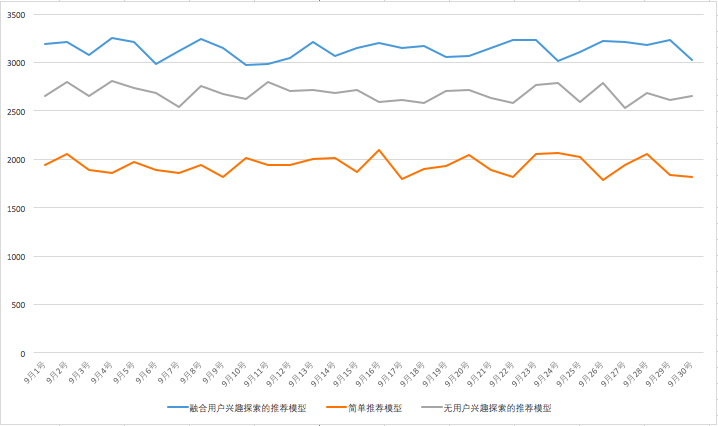
\includegraphics[scale=0.55]{figures/hl_themeNumber}}
    \figcaption{推荐多样性实验对比图}
    \label{pic:hl_themeNumber}
  \end{figure}

  我们对比了无兴趣探索模块的推荐模型、推荐热门商品的简单推荐模型和融合了兴趣探索模块的推荐模型在实验期间的点击购买转化率。\autoref{pic:hl_buyLookRatio}展示了不同模型的实验结果。图中,横坐标是时间变量,单位为天,纵坐标是点击购买转化率,每一条曲线代表了一个模型的点击购买转化率随时间变化的曲线。实验结果显示,融合了兴趣探索模块的推荐模型相对其他模型有更高的点击购买转化率。融合了兴趣探索模块的推荐模型的平均点击购买转化率是32.74\%,比推荐热门商品的简单推荐模型的平均点击购买转化率9.63\%要高,相对于无兴趣探索模块的推荐模型的平均点击购买转化率17.54\%也高了不少。由此可见用户兴趣探索能够很好的提升点击购买转化率。
  \begin{figure}
  \centering
    \framebox{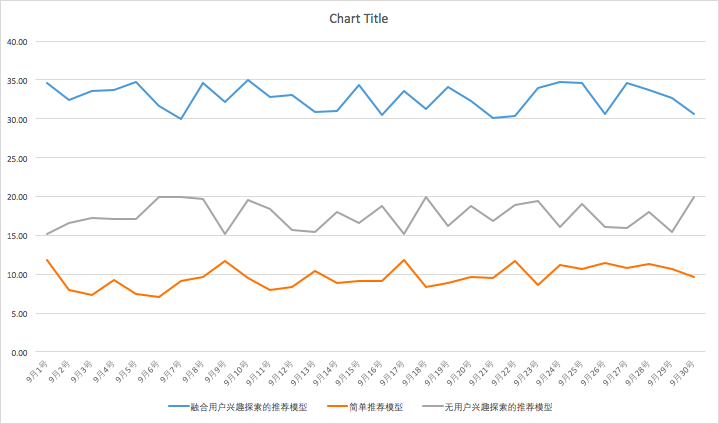
\includegraphics[scale=0.55]{figures/hl_buyLookRatio}}
    \figcaption{转化率实验对比图}
    \label{pic:hl_buyLookRatio}
  \end{figure}

\section{本章小结}
本章首先介绍了用户行为数据特点以及基于此的用户行为数据的的预处理。然后介绍了用户兴趣探索模块的组成内容,包括兴趣标签探测功能模块、长尾标签抽取功能模块和用户满意度量化功能模块,之后介绍了用户画像和用户兴趣探索的融合,最后给出了用户兴趣探索实验结果,即用户兴趣探索模块可以为推荐系统带来更好的多样性和更高的购买转化率。